\section{Introduction}
\label{sec:introduction}

% state the learning objective 

\hspace{0,5cm} This report is being made for the subject of Circuit Theory and Electronics Fundamentals and is related to the $1^{st}$ laboratory.

The objective of this laboratory assignment is to study a circuit containing seven resistors, one voltage source, one current source, one current controlled voltage source and one voltage controlled current source. The elementary meshes are named after the current to which they are attributed and so there are four of them.

The current controlled voltage source $V_c$ is calculated by multiplying $K_c$ with the current $I_c$, whereas the voltage controlled current source $I_b$ can be determined by multiplying $K_b$ with the voltage source $V_b$.

The display of this circuit can be seen in Figure~\ref{fig:circuito}.

In Section~\ref{sec:analysis} it will be analysed theoretically the circuit by both Nodal and Mesh Method ending with the presentation of the results obtained by Octave.

Secondly, in Section~\ref{sec:simulation} it will be simulated the circuit using ngspice, the results obtained will be presented and compared with the ones gathered from Section~\ref{sec:analysis}.

The conclusions of this study are outlined in Section~\ref{sec:conclusion}.

\begin{figure}[h] \centering
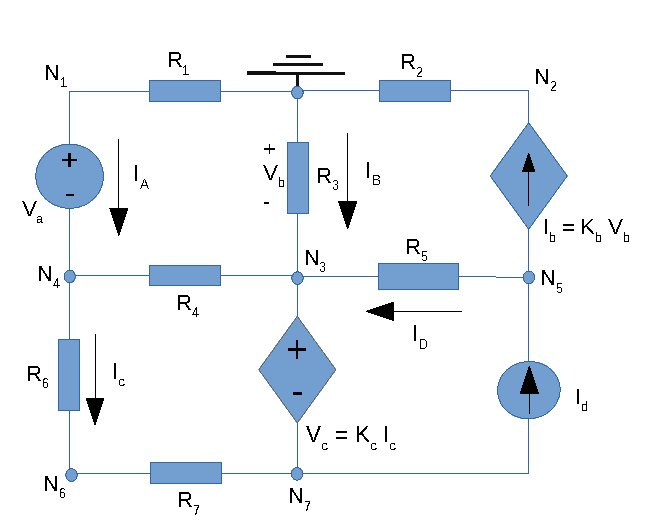
\includegraphics[width=0.7\linewidth]{circuito.pdf}
\caption{Circuit} %mudar legendaaaaaaaaaaa!!!!!!
\label{fig:circuito}
\end{figure}


\begin{center}
Where:

$R_1 = 1.03431507833 $

$R_2 = 2.02853090731$
 
$R_3 = 3.1462050633 $

$R_4 = 4.03438547455$ 

$R_5 = 3.12170042214 $

$R_6 = 2.07116379646 $

$R_7 = 1.01597753093 $

$V_a = 5.156959346 $

$I_d = 1.01455683569 $

$K_b = 7.1497941196 $

$K_c = 8.12593642585 $
\end{center}

The units of the elements whose name starts with R (the resistors) are $k\Omega$ (kiloohm), the ones that start with I are expressed in $mA$ (miliampere) and the ones starting with V are expressed in $V$ (volts). While Kb is given in $mS$ (milisiemens), Kc is also given in $k\Omega$.

These values where obtained using the \textit{Python} script using the lowest student number on our group - 95785.


